% chapter Design of Elib
\chapter{Elib design} \label{chap:elib}
  The {\it Elib} library is a $C\#$ asynchronous library for a remote control of e-Puck. 
  The goal of the library is to make developing programs for the robot easier.
  This chapter presents several topics, which influenced the design of {\it Elib}.
  The Examples on use of $Epuck$ class and its interfaces are introduced is in the ~\ref{chap:usage} Chapter.

  In the first place the possibilities of programming e-Puck are depicted.
  Next section covers the advantages and the drawbacks of asynchronous remote control programming of e-Puck.
  Furthermore, key features of {\it Elib} are presented together with crucial decisions, which
  lead to properties of {\it Elib}. 
  {\it Elib's} features are confronted with the alternatives. The differences are discussed
  and the main reasons for choosing the current implementations are mentioned.

  After that, the logic of the main classes $Sercom$ and $Epuck$ are introduced. Sections 
  \ref{sec:sercom} and \ref{sec:epuck} describe implementation of the classes in detail. 
  In the part devoted to $Sercom$ the main stress is on the design of Bluetooth communication processing.
  The implementation details of the two $Epuck's$ interfaces are the main topic of rest of this chapter. 

  The last Section \ref{sec:suminterface} sums up qualities of interfaces 
  implemented by $Epuck$ and $Sercom$ class.
  Section \ref{sec:suminterface} also describes {\it Elib's} performance results.

  This chapter assumes that a reader understands the use of callbacks and $EventWaitHandle$ class in .Net and.
  The callbacks and $EventWaitHandle$ class together with other advanced .Net features 
  are introduced in section ~\ref{sec:net}.

\section{Approaches to e-Puck programming} \label{sec:approach}
  E-Puck is distributed with several programs in its flash memory. 
  Most of the programs implement a simple behaviour, which introduces e-Puck sensors and actuators.
  There is a behaviour, which made e-Puck go to the source of light.
  If another behaviour is running, e-Pucks
  reacts to clapping and it turns around to source of a clap. An interesting behaviour makes
  e-Puck cry, if it is falling.
   
  The {\it BTCom} program and e-Puck bootloader are also distributed on e-Puck, but belong to different classes of programs. 
  {\it BTCom} allows e-Puck to communicate with other devices via Bluetooth.
  It defines a BTCom protocol, which works in two modes. The text mode accepts commands for
  all sensors and actuators except for the fact that it does not allows take a picture 
  with an e-Pucks camera. 
  The accepted commands and the sent answers of BTCom protocol are short text messages.
  On the other hand, {\it BTCom} in the binary mode can send a picture from e-Puck.
  If {\it BTCom} runs in the binary mode, commands in single bytes are accepted instead of text messages.
  The binary mode is more economical, 
  because the commands are sent in single bytes and also the integer values from sensors
  are not converted to a textual form.
  The binary mode of {\it BTCom} does not control all sensors and actuators, because it accepts fewer commands than the text mode.
  The absence of commands for controlling some sensors and actuators is the main reason 
  for sending all commands from {\it Elib} to {\it BTCom} in the textual form. 
  The single exception is sending an image back to {\it Elib} in the binary mode.
   
  Bootloader, officially called Tiny Bootloader\cite{tiny}
  , is the only wired program on e-Puck. It downloads	other programs to e-Puck via Bluetooth. 
  Tiny Bootloader has its counterpart, a graphical PC application,
  which allows users easy download hex files to e-Puck.
  A hex file\footnote{\small{\url{http://en.wikipedia.org/wiki/Hex_file}}} 
  for e-Puck is compiled C program for e-Puck's dsPic microchip. 
   
  All mentioned programs including Tiny Bootloader use a C library, which interface the devices on e-Puck. 
  The library and the programs are published under open source licence at
  \url{http://www.e-puck.org}.

   
  If e-Puck is turned on, e-Puck starts running one of the downloaded programs according a selector 
  position. E-Puck's selector switch is located on the main board of e-Puck.
  If a programmer wants to run another program, he has to switch selector to another position
  and hold a second a reset button on e-Puck.	Selected program is loaded from flash memory
  to RAM memory and immediately executed.	
   
  Suppose there is correct C code for e-Puck's processor saved on PC. What has to be done to run the program?
  Let us describe the procedure.
  Firstly it has to be compiled and linked. After that transformation to a hex file is necessary,
  because e-Pucks's dsPic is 16 bit processor. In next step turn Bluetooth and e-Puck are turned on. 
  The robot and your computer are paired together. The user has to enter the PIN, 
  which is needed to pair the devices 
  PIN is a number, which is on e-Pucks body.
  The OS opens a serial port for Bluetooth communication.
  Graphical counter part of Tiny Boatloader is needed. It is used to select the hex file and choose the opened port. 
  Furthermore, the Tiny Boatloader guides user through the downloading of the hex file.
  The instructions tell the user to press a reset button on e-Puck. It has to be pressed only for about a second.
  Tiny Bootloader announces when the download finishes. To run the program it is necessary to to reset e-Puck.
   
  The program is written to e-Puck's flash memory according e-Puck's selector position.
  If another program had been saved under the same selector position, it is overwritten by the new program.
  Downloading of hex file to e-Puck last usually approximately 30 seconds and quite often is unsuccessful. 
  Programming e-Puck via Tiny Boatloader is not very comfortable. 
  Luckily, there is an another way, which uses {\it BTCom}. 

  In order to use {\it BTCom} turn selector to position, under which it is downloaded, and press reset button.
  Now {\it BTCom} is running.  Pair your PC with e-Puck as described above and use the open port
  to control e-Puck.
  {\it BTCom} starts running in text mode, so its possible to use a terminal to communicate with e-Puck.
  E.g Hyperterminal on Windows. On Linux write directly to the serial port using a command line.
  A program can control e-Puck via BTCom protocol too, but it must process the commands ant their replies.
   
  Nice example of accessing sensors and actuators over Bluetooth is 
  e-Puck Monitor\footnote{\small{Download E-Puck Monitor from \url{http://www.e-puck.org}.}}.
  E-Puck Monitor is an open source graphical application written in C++, which uses BTCom protocol. 
  It can send and process answers to every sensor and actuator.
  It presents values of all sensors on one screen. Actuators can be controlled by mouse or by inserting
  proper values into text boxes.

  E-puck Monitor's serious drawback is its freezing. The application does not respond, 
  because it waits synchronously to answers from {\it BTCom}.
  If a Bluetooth connection with e-Puck is broken or the answer is lost, the application stays unresponsive.
   
  Downloading a hex file to e-Puck's microchip and remote control over BTCom protocol are two alternatives
  of controlling e-Puck.
  Using {\it BTCom} user do not have to download any file to e-Puck's microchip.
  It is great advantage, because the length of developing cycle of program to e-Puck's processor is reduced.
  The developing cycle consist of	writing a code, compiling it, downloading it, debugging it and correcting it.
  In following section the drawbacks will be described in detail and it will be confronted with
  remote control.
\section{Advantages of remote control} \label{sec:remote}
  The applications, which use {\it BTCom} and its protocol, run a whole algorithm on PC and {\it BTCom} just 
  execute the commands and get the values from sensors. Imagine you have a library, which process the commands
  and their replies. Your program uses the library and just asks the library for sensor values and
  gives the library commands what to do. The life cycle of developing a program is still writing a code, 
  compiling it, debugging and rewriting. Important is that downloading part is missing.
   
  It is so important, because downloading a program to e-Puck takes the most time and is the most 
  unreliable part of the life cycle except debugging.
  The quality of debugging also differs a lot between these two attitudes.
   
  If a program is downloaded to e-Puck, there are only e-Puck's actuators for a feedback.
  The actuators are a very poor debugging tool, because if something goes wrong, 
  it is impossible to say if the program stopped running,
  or e-Puck is waiting to sensors values, or battery is down. 
  Discovering the problem, even if it is the low battery, takes one or two loops of downloading and compiling the program.
  E-Puck still has the indicator of battery, but it is not reliable.
  Downloading a program takes a long time and successful download could last even a couple of minutes. 
  It drives a lot of people crazy.
   
  A programmer, which controls robot remotely, can of course debug with tools of his programming environment and much more.
  He is able to use e-Puck's sensors too. Also his own logging program can be useful. 
  All this can be utilised, because a computer has usually much more resources than e-Puck has.
  A developer has all variables under control. If he set the breakpoints
  right, the logic should not be damaged. 
  The breakpoint damages the logic of application only if it is set between two commands,
  which first has sent a command and the second is waiting to it.
  Furthermore, other sensors connected to his computer could help.
  
  If the remote control is used, it can be said that the intelligence 
  is located on a computer. However if you load a program to e-Puck via Tiny Bootloader the whole algorithm
  runs on e-Puck.
   
  The resources of PC are useful first of all for implementation of the program and not only for
  its debugging. E-Puck for example takes pictures smaller than 3200 bytes, complicated image processing still
  requires too much work for e-Puck's microchip. It is faster to process the picture
  on a computer. Let us note that also implementing a neural network or even genetic algorithm on 8kB memory
  is very difficult.
\section{Design of {\it BTCom} program. What does it mean for {\it Elib}?}
  \label{sec:btcomdesign}
  The interfaces of {\it Elib} is designed for {\it BTCom} version 1.1.3, but {\it Elib} is also compatible with {\it BTCom} 2.0.
  The complete {\it BTCom} source code is located on enclosed CD in file "btcom.c".
  Let us note that we added some comments to the source code. Original comments begin with two slashes,
  our comments starts with four slashes.

  {\it BTCom} is a mainly textual protocol, which is defined by {\it BTCom} program. The answer of {\it BTCom} always begins 
  with the first letter of the relevant command.
  If the command requires some sensor values, the value is attached to the first letter and
  sent. Otherwise the first letter of command is sent back alone. Each answer ends by 
  $\backslash$r$\backslash$n escape sequence.
  List of all text commands available see below.
  \lstset{basicstyle=\small}
\begin{lstlisting}
"A"         Accelerometer
"B,#"       Body led 0=off 1=on 2=inverse
"C"         Selector position
"D,#,#"     Set motor speed left,right
"E"         Get motor speed left,right
"F,#"       Front led 0=off 1=on 2=inverse
"G"         IR receiver
"H"          Help
"I"         Get camera parameter
"J,#,#,#,#" Set camera parameter mode,width,heigth,zoom(1,4,8)
"K"         Calibrate proximity sensors
"L,#,#"     Led number,0=off 1=on 2=inverse
"N"         Proximity
"O"         Light sensors
"P,#,#"     Set motor position left,right
"Q"         Get motor position left,right
"R"         Reset e-puck
"S"         Stop e-puck and turn off leds
"T,#"       Play sound 1-5 else stop sound
"U"         Get microphone amplitude
"V"         Version of BTCom
\end{lstlisting}
    
    
  Let $A$ be a PC and $B$ be an e-Puck robot. $A$ controls $B$ over BTCom protocol. {\it BTCom} program located on $B$ 
  replies to all commands sent from $A$.
  The answers of {\it BTCom} from $B$ allows $A$ to know that the sent command was received and
  executed. 
   
  Two main questions, which effect design of {\it Elib}, arise from the {\it BTCom} structure.
  Should {\it Elib} limit the waiting time for an answer from $B$?
  How fast should {\it Elib} allow $A$ sending the commands to $B$?
   
  At first let us stress that sending commands from {\it Elib} does mean in the following paragraphs
  sending textual or binary commands
  using {\it BTCom}. It does not mean calling any functions of the {\it Elib} library, which wrap the sending. 
   
  It is necessary to understand, that not only executing a {\it BTCom} command, 
  but also a transfer of a command and a transfer of reply take insignificant amount of time. 
  The time is measured from a computer processor's point of view, because
  it is the processor, who is waiting to serial port, which is sending the message.
   
  Back to the question how should {\it Elib} limit sending of the commands.
  As we have said sending commands takes a while and therefore sending is performed asynchronously. 
  Due to asynchronous sending, users do not have to wait to the end of sending previous command and
  can send next before the first command has finished.
  It leads to queueing the commands in a serial port output buffer of PC. Unfortunately the buffer is usually not 
  very large and can easily overflow. 
  This is the reason for implementation {\it Elib's} buffer, a queue, which slows down the sending and does not allow
  overwriting of sent commands by each other in the output buffer. 
   
  Is problem with sending solved? Not for e-Puck. If the commands were sent too fast,
  the input buffer of e-Puck would have the same problem, because e-Puck's processor does not keep up emptying e-Puck's
  input buffer. The buffer would be flooded and the commands would be overwritten. 
  {\it Elib} has to check, if the Bluetooth is not able to send commands too fast for e-Puck
  and possibly slow down sending of commands even more.

  %How fast can e-Puck receive commands? Experiments showed, that gaps between commands around 0.02 s are 
  %critical at best condition, because e-Puck processes each answer immediately as it picks it up from its input buffer.
   
  Let us focus on how long {\it Elib} should wait to the answer.
  Clearly we have to wait more than is the minimum transfer time from a computer to e-Puck and also
  the transfer time of the answer.
  The times of answers are all almost identical for actuators and corresponds with times for sending commands.
  Sensors messages carries more data on the way back, therefore sending sensors answers take longer time.
  An extreme is a command for taking a picture. Sending command to e-Puck last about 0.02 s, but
  the answer needs more than 0.2 s for a transfer.
   
  As we mentioned, waiting for the answers takes even longer time than sending a command,
  so the waiting is performed in {\it Elib} asynchronously too.
   
  Due to asynchronous design we can afford to wait as long as we can. 
  Possible variability of waiting time force {\it Elib} to let the user decide how long
   {\it Elib} should wait for an answer. The {\it Elib} library does not limit the minimum waiting time,
  because the convenient values differs according a state of a battery on e-Puck, a strength of Bluetooth signal
  and many others factors. 
  
  In examples, which are introduced in Chapter ~\ref{chap:usage}, the waiting times are set to the bottom values,
  which allow commands to be confirmed without no problems under good conditions.
  The waiting times for answers are in {\it Elib} called $timeouts$.
   
  Let us sum up the facts. Sending of commands takes insignificant amount of time.
  Sending commands are queued, because otherwise they could be overwritten in the buffers.
  Receiving an answer takes even more time than sending a command from computer.
  We concluded to implement sending commands and receiving answers asynchronously, because the communication with e-Puck
  can be pointlessly holding up a processor of PC.
  What means asynchronous implementation in case of {\it Elib}? What is done if the answer receives in time
  and what if not? These questions are answered in next section called Asynchronous programming model for {\it Elib}.
\section{Asynchronous programming model (APM)\\ for the {\it Elib} library}
  \label{sec:apm}
  It was already mentioned that an asynchronous call of a function is convenient if the
  classical synchronous call let the processor waiting for instance to a device.
  In e-Puck's case the device is serial port. 
   
  There is an synchronous communication using {\it BTCom} implemented in Epuck Monitor
  \footnote{\small{Download at \url{http://www.gctronic.com/files/e-puckMonitor_2.0_code.rar}}}. 
  Epuck Monitor waits not only to send the commands, but also it waits synchronously on the answers.
   
  Graphical applications usually explicitly require to stay responsive. 
  If they are not responsive, they freeze like Epuck Monitor.
  On the other hand, asynchronous programming is much more complicated than synchronous programming.
  The goal of {\it Elib} is to hide the complications of APM and offer an interface
  which performs sending and receiving messages asynchronously and
  which allows a programmer to easily create applications for e-Puck. For example applications like Epuck Monitor.
   
  {\it Elib} has two main classes and two interfaces implemented.
  $Serom$ is a public class which wraps serial communication.
  $Epuck$ class represents an instance of a e-Puck robot and uses $Sercom$ internally.
  The interface of $Sercom$ for sending commands takes a
  string command, two functions, class object and an integer as its arguments.
  The string specifies a type of command. The integer represents the $timeout$.
  The first function is called if the answer is delivered in time.
  The second function is called if the $timeout$ has elapsed and the answer has not arrived.
  The second function also uses the class $object$ as its argument.  These described
  functions are in {\it Elib} called $Okf$ and $Kof$ callbacks. The class $object$
  can be used to send information for the function, or to gain information from the called function.
  Callbacks are functions, which are called after some procedure has finished.

  $Epuck's$ commands have two interfaces. First is directly based on the interface of 
  the $Sercom's$ $Write(..)$ function and it only removes the string argument which the functions
  implement implicitly.
  Let us call it a basic interface.
  The second interface of commands is based on the basic $Epuck's$ interface. 
  It also accepts $timeout$, an instance of $object$ class and one callback, but it returns 
  an implementation of $IAsyncResult$ interface which will be introduced later.
  Simpler interface logic	and the fact that $IAsyncResult$ is well known interface
  are reasons for implementing the $IAsyncResult$ interface.
  %The interface is used across different .Net libraries.

\begin{figure}[!hbp]
\begin{lstlisting}[language=cs]
public class Sercom {
  public void Write(string command, RCallback okf, NRCallback kof,object state, double timeout) {
          //... the body of function
  }
}
public class Epuck {
  public void Stop(OkfActuators okf, NRCallback kof, object state, double timeout) {
          //example of interface directly based on BTCom's interface
  }
  public IAsyncResult BeginStop(double timeout, AsyncCallback callback, Object state) {
          //example of IAsyncResult interface implementation
  }
}
\end{lstlisting}
\caption{Public methods of $Sercom$ and $Epuck$} \label{serep}
\end{figure}
\section{The $Sercom$ class}\label{sec:sercom}
  An instance of $Sercom$ allows a computer to asynchronously communicate with other devices
  over serial communication. The class accepts textual commands and parses textual answers.
  The commands and answers can be distinguished according its first letter.
  
  Every sent command waits until the answer arrives or its $timeout$ elapses.
  After that next command is sent. Let us is called this kind of waiting a $handshaking$ hereafter.

  This implementation automatic guarantee that the commands would not be sent too fast,
  because $Sercom$ waits on e-Puck's answer. E-puck picks up the command from its input buffer and then sends the reply.
  The short answers under good conditions make do not slow down sending with $handshaking$, because
  they arrives under 0.04. For example the "stop" command has been confirmed under 0.04 s in all 20 attempts.

  $Handshaking$ solves the problem with synchronising sending and receiving the commands and their answers. 
  It made us choose $handshaking$ as the best implementation.

  E-Puck processes a received message in three steps. It picks the command from input buffer.
  It process the command and then reply with an answer.
  For commands with long sending or processing phase it means following consequence.
  If such command is sent, next commands has to wait longer time, because there is a
  danger of e-Puck's input buffer overflow.

  %todo ulehcit ctenarovi cteni, tezko citelne
  At the beginning of a {\it Elib's} development we thought about implementing both the $handshaking$
  and the $nonhandshaking$ sending.
  The $nonhandshaking$ sending does not wait to answer of the previous command. It sends the next command immediately. 
  Motivation for $nonhandshaking$ is to save time which is spent on waiting to the answers of the sent commands.
  Consequently $nonhandshaking$ has to ensure that the input buffer does not overflow.
  We have experienced that it is a nontrivial task to set the correct time gap after different types of commands. 
  The final observation is that the $nonhandshaking$ sending is even slower than the $handshaking$ sending, 
  because the gaps after sent commands have to be set at maximum in order to avoid a failure under all conditions. 
  The gaps in $nonhandshaking$ mode has too be exorbitant, %todo naddimenzovany
  because it must not to let the input buffer of e-Puck overflow.

  Next advantage of $handshaking$ is its simple and elegant implementation. It also does not depend on {\it BTCom} implementation so much.
  If {\it BTCom} had improved the times of processing the answers,
  in $nonhandshaking$ mode it would have resulted into a change of table, which stores minimal gaps after each command.



  \subsection{The logical problems with a confirmation of commands}\label{sec:logical}
  In $nonhandshaking$ mode a lot of commands can be sent before the $timeout$ of the first elapses.
  Let us introduce a common situation, which causes a serious problem. 
  
  Let the sent commands be of one type. For example all the commands can control the front LED light.	
  The problem consist of unwanted postponing a call of the $Kof$ callback. 
  Let us imagine that the answer to first command
  is lost, but the second answer manage to be processed under $timeout$ of the first command.
  It means that $Okf$ callback is called and the user assumes that everything is fine.
  Furthermore, the problem can be postponed to the last command of the same type,
  because the reply to the second command can be substitute for the reply of the third command
  and so on.

  The commands can be logically different, although they are of the same type.
  The $Kof$ callback can be called on a different command, because the first command can turn the front LED on 
  with message "F,1", however the last command can switch the front led off with "F,0" command and 
  the reply to both commands is "F$\backslash r\backslash n$.

  $Handshake$ mode does not suffer from calling the wrong callback, however if the $Kof$ callback
  does not prevent the user program from a sending the command for the same device again,
  the answer from previous command can substitute the answer from the second command.
  The solution for a callback is to paste a command of a different type which will exclude the option
  of the interchange of the answers.

  A convenient tool of separation commands of same type is pasting the stop command between them.
  If the program is not sure, whether the robot is reacting to its commands, safe behaviour is to stop.
  If $Kof$ callback is called on stop command, sending the stop command again does not breaks the logic,
  because whichever answer confirms that e-Puck is stopped. More examples of implementing $Kof$ callbacks
  are described in Chapter ~\ref{chap:usage}.
\subsection{The current and the previous $Sercom's$ implementation}\label{sec:versions}
  The current $Sercom's$ implementation has only four public functions.
  The constructor, the $Start$ method, the $Dispose$ method and the public method $Write$. 
  See its interface in Figure ~\ref{serep}.	

  The previous versions of {\it Elib} in addition have implemented public method for changing from $nonhandshake$ mode to 
  $handshake$ mode and vice versa.

  The reason for introducing the previous versions with $nonhandshake$ implementation is to present 
  the inner implementation which is not dependent on $handshaking$ and $nonhandshaking$.
  %todo opravit simpler formulation nepekna
  We describe it, because it has simpler design, but the demands of resources increase rapidly, if a lot of commands are sent.
  The current implementation remains stable.
\subsection*{Previous version}\label{previous}
  In  Figure ~\ref{pic:sercom_nohandshake} the schema of the inner implementation 
  from the previous versions of {\it Elib} is illustrated.
  It shows functions and objects, which are used for sending and receiving the messages.
  Some methods have $nonhandshaking$ and $handshaking$ versions.
  $Nonhadshaking$ methods, which are drawn in red	in Figure ~\ref{pic:sercom_nohandshake}, implement the same logic 
  as $handshaking$ methods except they allow to send and receive more commands
  at once.

  %\input{sercom_nohandshake.TpX}
  \begin{figure}[!hbp]
  \centering
  \ifpdf
    \setlength{\unitlength}{1bp}%
    \begin{picture}(319.36, 236.63)(0,0)
    \put(0,0){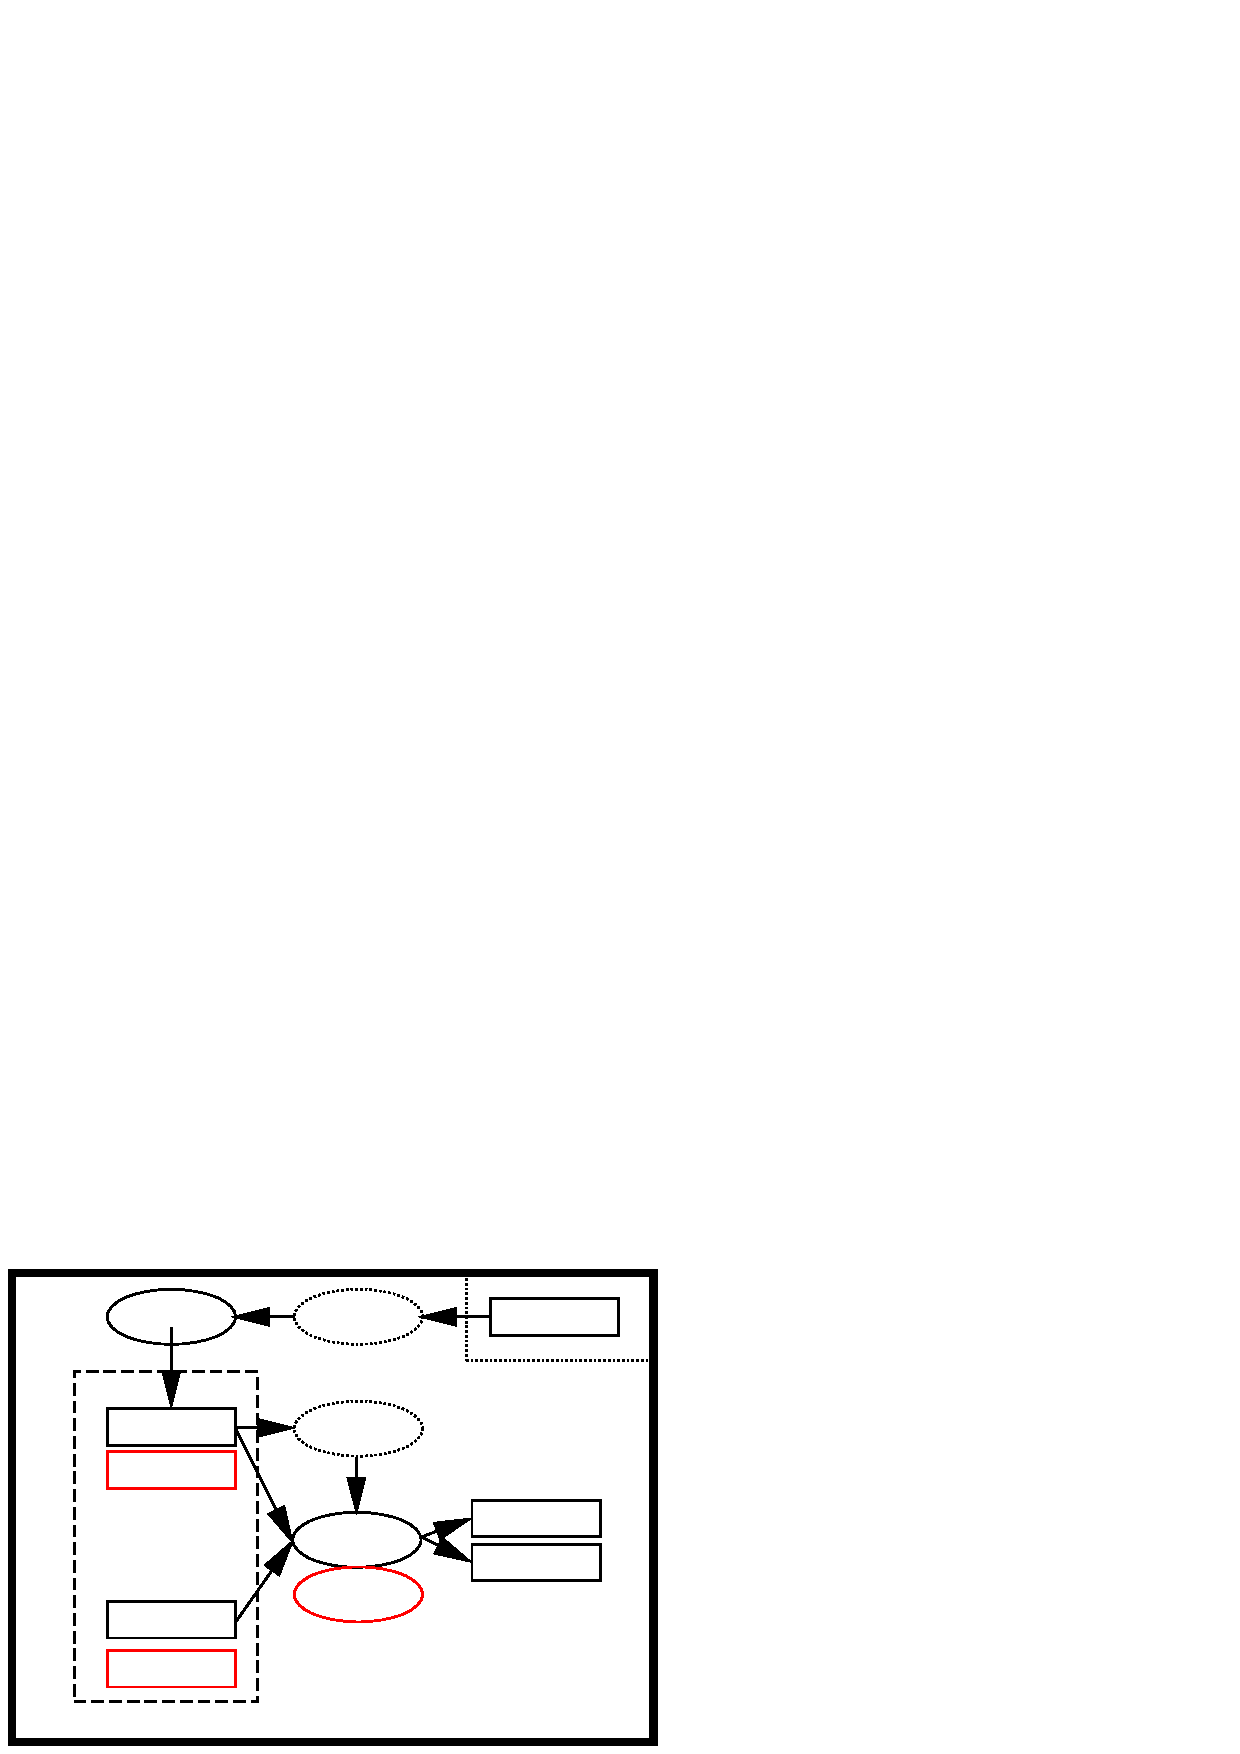
\includegraphics{sercom_nohandshake.pdf}}
    \put(41.75,105.11){\fontsize{5.30}{6.36}\selectfont These methods work with Serial Port.}
    \put(238.00,207.20){\fontsize{8.83}{10.60}\selectfont public Write(..)}
    \put(153.42,153.66){\fontsize{8.83}{10.60}\selectfont notSended}
    \put(153.42,207.34){\fontsize{8.83}{10.60}\selectfont notSended}
    \put(63.66,207.34){\fontsize{8.83}{10.60}\selectfont notSended}
    \put(60.73,61.89){\fontsize{8.83}{10.60}\selectfont  ~Receive(..)}
    \put(60.73,38.33){\fontsize{8.83}{10.60}\selectfont \textcolor[rgb]{1, 0, 0}{hReceive(..)}}
    \put(66.10,154.40){\fontsize{8.83}{10.60}\selectfont  ~Send(..)}
    \put(66.10,133.67){\fontsize{8.83}{10.60}\selectfont \textcolor[rgb]{1, 0, 0}{hSend(..)}}
    \put(238.00,207.20){\fontsize{8.83}{10.60}\selectfont public Write(..)}
    \put(153.42,207.34){\fontsize{8.83}{10.60}\selectfont notSended}
    \put(63.66,207.34){\fontsize{8.83}{10.60}\selectfont notSended}
    \put(229.20,89.27){\fontsize{8.83}{10.60}\selectfont Checker.Okf(..)}
    \put(229.20,110.39){\fontsize{8.83}{10.60}\selectfont Checker.Kof(..)}
    \put(155.29,100.33){\fontsize{8.83}{10.60}\selectfont  ~Sent [c]}
    \put(161.97,74.11){\fontsize{8.83}{10.60}\selectfont \textcolor[rgb]{1, 0, 0}{hSent}}
    \end{picture}%
  \else
    \setlength{\unitlength}{1bp}%
    \begin{picture}(319.36, 236.63)(0,0)
    \put(0,0){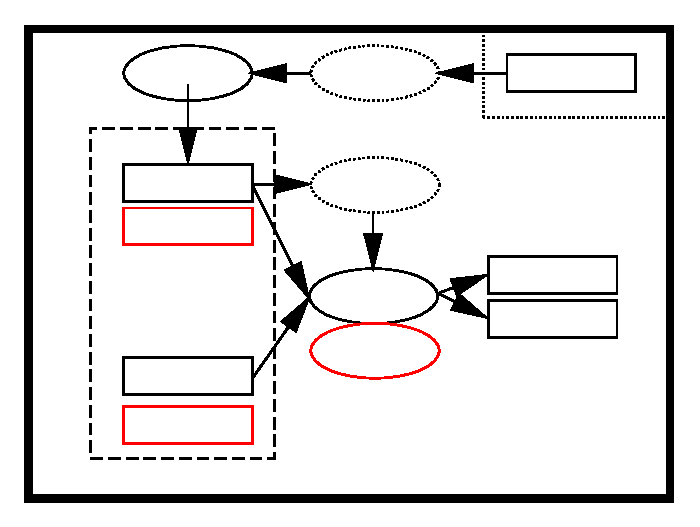
\includegraphics{sercom_nohandshake}}
    \put(41.75,105.11){\fontsize{5.30}{6.36}\selectfont These methods work with Serial Port.}
    \put(238.00,207.20){\fontsize{8.83}{10.60}\selectfont public Write(..)}
    \put(153.42,153.66){\fontsize{8.83}{10.60}\selectfont notSended}
    \put(153.42,207.34){\fontsize{8.83}{10.60}\selectfont notSended}
    \put(63.66,207.34){\fontsize{8.83}{10.60}\selectfont notSended}
    \put(60.73,61.89){\fontsize{8.83}{10.60}\selectfont  ~Receive(..)}
    \put(60.73,38.33){\fontsize{8.83}{10.60}\selectfont \textcolor[rgb]{1, 0, 0}{hReceive(..)}}
    \put(66.10,154.40){\fontsize{8.83}{10.60}\selectfont  ~Send(..)}
    \put(66.10,133.67){\fontsize{8.83}{10.60}\selectfont \textcolor[rgb]{1, 0, 0}{hSend(..)}}
    \put(238.00,207.20){\fontsize{8.83}{10.60}\selectfont public Write(..)}
    \put(153.42,207.34){\fontsize{8.83}{10.60}\selectfont notSended}
    \put(63.66,207.34){\fontsize{8.83}{10.60}\selectfont notSended}
    \put(229.20,89.27){\fontsize{8.83}{10.60}\selectfont Checker.Okf(..)}
    \put(229.20,110.39){\fontsize{8.83}{10.60}\selectfont Checker.Kof(..)}
    \put(155.29,100.33){\fontsize{8.83}{10.60}\selectfont  ~Sent [c]}
    \put(161.97,74.11){\fontsize{8.83}{10.60}\selectfont \textcolor[rgb]{1, 0, 0}{hSent}}
    \end{picture}%
  \fi
  \caption{\label{pic:sercom_nohandshake}%
   Old structure}
  \end{figure}


  Sending a command starts with calling public method $Write$. The instance of $checker$ class is created in the $Write$ method.
  $Checker$ stores the command name, $Okf$, $Kof$, a reference to $state$ object and references to $notSent$ 
  and $Sent$ queues.
  It also stores a boolean value $answered$, which indicates whether the answer has been already delivered or not.

  $Checker$ starts a separate thread in the $Write$ method. In the thread runs the $check$ method, which at first sleeps for a $timeout$.
  After the $timeout$ expires a method the $check$ method finds out whether the answer has arrived.
  If $answered$ has been set to true, it means that the $Okf$ callback has already been 
  called and nothing is done. In other case, $Kof$ is called and $answered$ is set to $true$.

  Let us introduce methods which send and receive commands.
  $Send$ respectively  the $hSent$ method and $Receive$ respectively the $hReceivve$ method run in a worker thread. 
  Method $hSent$ dequeues an instance of $checker$ class from $notSent$ queue and
  sends the command as soon as possible. The $hSent$ method waits until the $hSent$ variable
  of previous command is set to $null$. Both methods move the instance
  of $checker$ class from $notSent$ to $Sent$ respectively to $hSent$ after sending the command.

  $Sent$ is a queue of the $checker$ objects, $hSent$ is a reference to the $checker$ object. 
  
  \label{p:oneargument}
  The $Receive$ method process the text messages from the serial port and if a whole command is received
  it finds the first relevant instance of  $checker$.
  The answer is passed as one of the arguments to $Okf$ function and the function is called.
  If there is no $checker$ instance, which carries the same type of command with received answer,
  the answer is thrown away.

  $Okf$ delegate for the functions has additional string arguments for the answer, because the sensors answers contain values
  which the functions use after they are called.
  $Kof$ function has nothing to process, therefore it implements only the $state$ argument 
  which is also available in $Okf$ functions. The $state$ argument serves to retrieving
  some other information from the callback functions, although it can be also used for
  passing the information through the $state$ object into the callback method.

  The $checker$ instance of each sent command is during its existence saved either in the $notSent$
  queue or in the $Sent$ queue, respectively in the $hSent$ variable.
  After calling the $Okf$ or the $Kof$ functions the $checker$ instance is removed either from $notSent$ queue
  or from $Sent$ queue, respectively from $hSent$ variable. 

  This design cumulates threads. For each command in $notSent$ queue there is 
  one thread sleeping in $check$ method. If the sending is slow, the commands and its $checker$ objects are queued in
  $notSent$ together with their sleeping threads. Threads are valuable system resources. 

  It can be sent and received more than 20 commands per second and the longest $timeout$ for 
  e-Puck reset has to be at least 1.5 second, so more than 30 commands can be easily created.
  If the {\it Elib} is used improperly, for example thousand of commands are sent and its $timeout$ elapses
  in the same time, then thousand of threads is need. This design of {\it Elib} is inconvenient, because
  it uses abundant number of system resources.

\subsection*{The current $Sercom$}\label{sec:current}
  The current version abandoned the implementation of the $nonhandshaking$ mode, 
  because of the problems with receiving answers described 
  in section ~\ref{sec:approach}.
  It also solves the problem with	redundant threads. 
  
  {\it Elib} currently uses two working threads and implements only the $handshake$ mode.
  One thread running in the $checkNS$ function checks whether the $timeout$ of sent commands
  has not elapsed during waiting in $notSent$ queue. The second thread checks whether the sent command
  stored in the $hshake\_sent$ variable has a valid $timeout$ or the $timeout$ has already elapsed.
  $Send$ calls asynchronously $AsyncSend$ function, which dequeues an instance of $ansGuard$ from $notSent$ queue.
  The $ansGuard$ class is a wrapper of commands like $checker$ in the older versions and it will be presented below.
  The answers are also read asynchronously in the $DataReceived$ procedure.

  Both methods $Send$ and $DataReceived$ use a so called .Net asynchronous
  delegate invocation. It enables simple asynchronous invocation using a minimum resources.

  Let us briefly describe an instance of $ThreadPool$ class, which is created at 
  start of the application. It prevents from useless thread creation. The instance of the class keeps the threads after 
  a function finish. The threads switch between different functions, which are called 
  by asynchronous delegate invocation.
  
  $ThreadPool$ uses a delegate to invoke the functions in different threads.
  Delegate\cite{delegate} is a .Net strictly typed wrapper for function instances.
  An example of asynchronous function invocation using .Net delegate is depicted in Figure ~\ref{invocation}.
  
\begin{figure}[!hbp]
\begin{lstlisting}[language=cs]
// The form of delegate declaration garantees, that only functions
// with no arguments and with void returning value 
// can be saved in SendAsync delegate.
delegate void SendAsync();
void Send(object Sender, EventArgs ev) {
  //SendAsyncCall is a function, asyncCaller a delegate variable
  SendAsync asyncCaller = new SendAsync(SendAsyncCall);
  asyncCaller.BeginInvoke(null, null);      
}
// This function match requirements of SendAsync delegate.
void SendAsyncCall(){
  //the body
}
\end{lstlisting}
\caption{Example of Asynchronous function invocation}\label{invocation}
\end{figure}


  The $Sercom$ inner structure is based on the structure from previous versions, although
  different strategy is used to send commands, receive answers and check $timeouts$.
  All commands are wrapped by the $ansGuard$ class. An instance of $ansGuard$ is created in the $Write$ method.
  The references of callbacks are stored in $ansGuard$ together with their $state$ argument.  
  The $timeout$ value in seconds is added to the current time and stored in $ansGuard$.
  The instance of $ansGuard$ is immediately enqueued in the $notSent$ queue.
  All mentioned informations are saved to the instance of $ansGuard$ in the $Write$ method.

  The queue $notSent$ implements an event $NonEmpty$, which calls the $Send$ method whenever something is written
  to $Sercom$ by the $Write$ method. The $Sent$ method is also called, if the $hshake\_sent$ variable is set to $null$.
  $Send$ just calls $SendAsyncCall$. See a snippet in ~\ref{invocation} .

  Does $SendAsyncCall$ implement $handshaking$ mode?
  $SendAsyncCall$ actually does not send anything. It checks whether the command is received. 
  If $hshake\_sent$ is set to $null$ and the $notSent$ queue
  contains some $ansGuard$, then $SendAsyncCall$ moves $ansGuard$ from $notSent$ to $hshake\_sent$
  queue and sends the command. 

  %\input{sercom_handshake.TpX}
  \begin{figure}[!hbp]
  \centering
  \ifpdf
    \setlength{\unitlength}{1bp}%
    \begin{picture}(319.35, 257.75)(0,0)
    \put(0,0){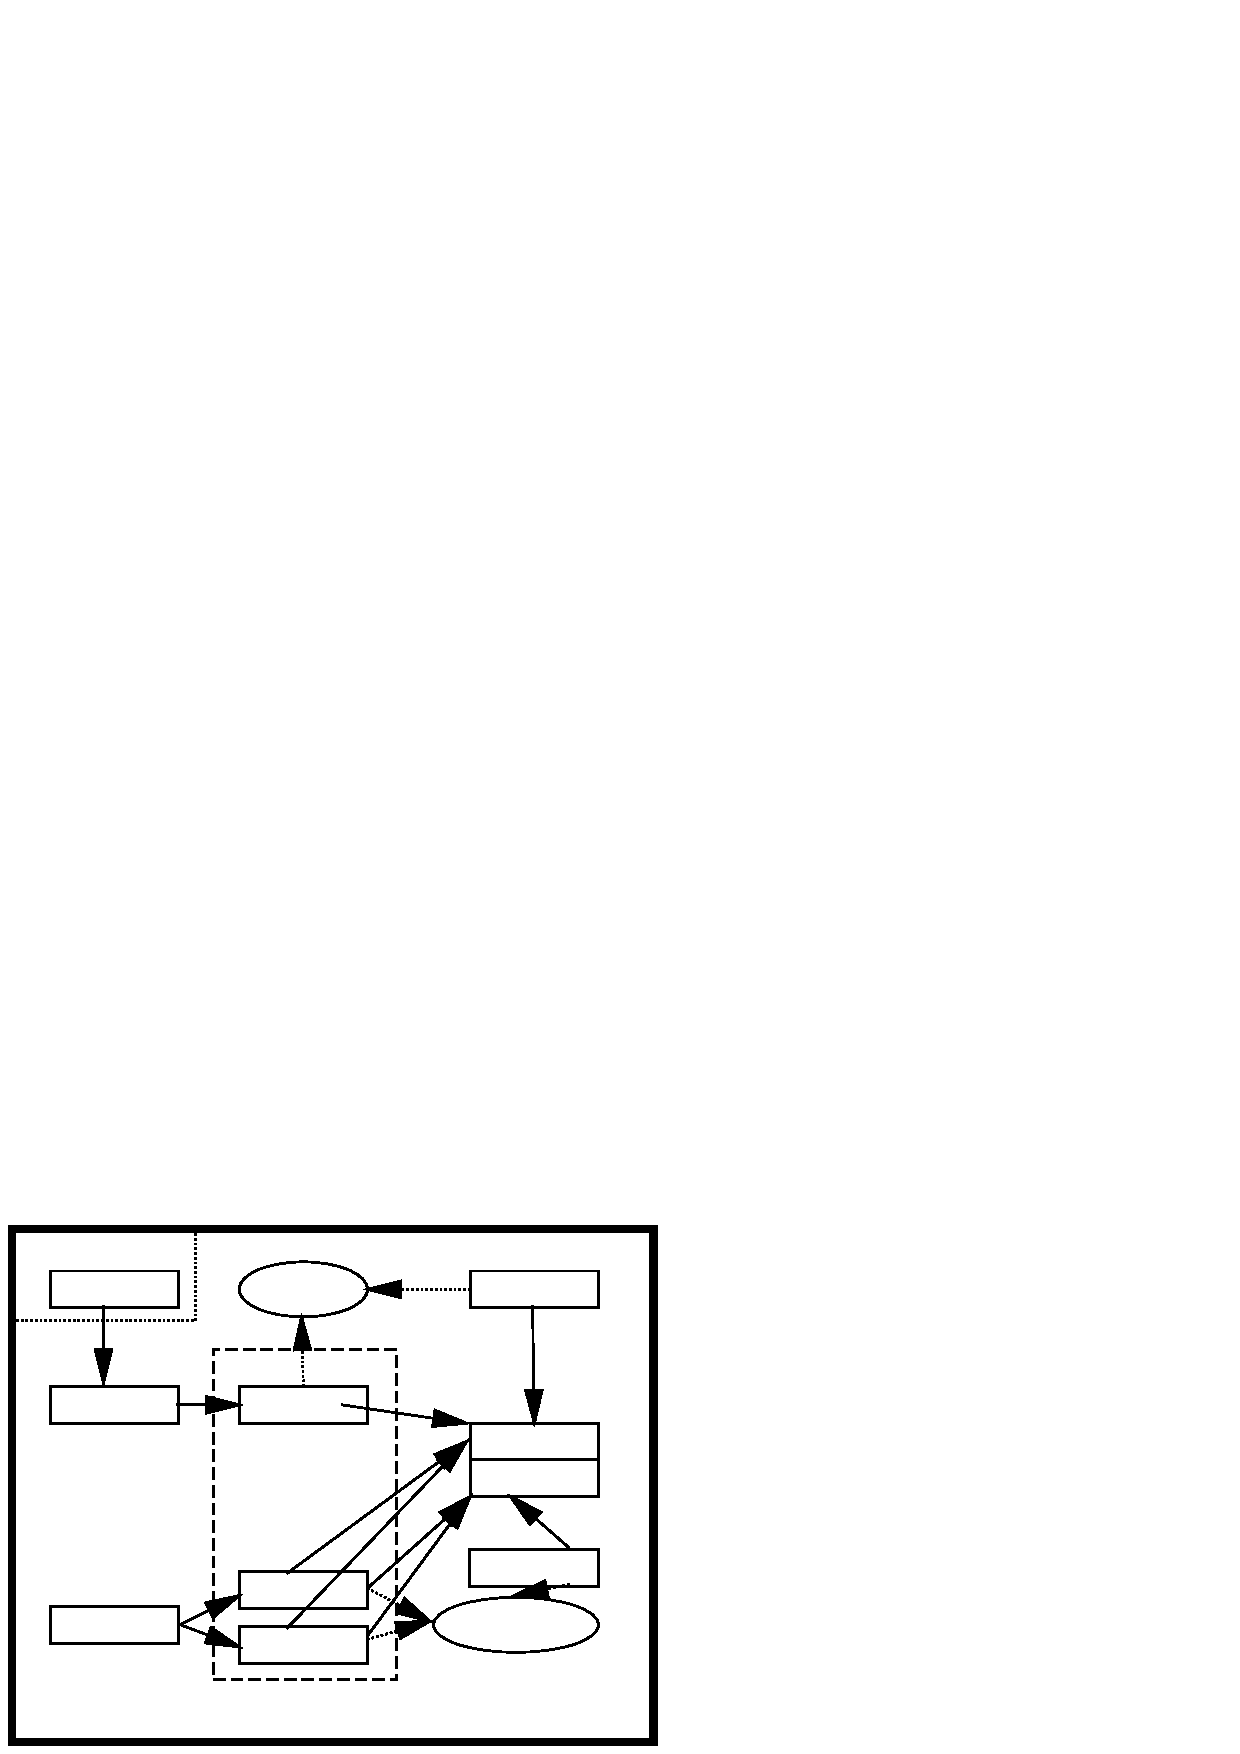
\includegraphics{sercom_handshake.pdf}}
    \put(117.44,49.67){\fontsize{7.07}{8.48}\selectfont BinaryModeRead(..)}
    \put(117.44,76.07){\fontsize{7.07}{8.48}\selectfont TextModeRead(..)}
    \put(127.02,220.54){\fontsize{8.83}{10.60}\selectfont notSent}
    \put(225.68,59.49){\fontsize{8.83}{10.60}\selectfont hshake\symbol{95}sent}
    \put(108.63,115.68){\fontsize{5.30}{6.36}\selectfont These methods work with Serial Port.}
    \put(26.79,59.35){\fontsize{8.83}{10.60}\selectfont Read(..)}
    \put(117.44,164.96){\fontsize{8.83}{10.60}\selectfont AsyncSend(..)}
    \put(26.79,164.96){\fontsize{8.83}{10.60}\selectfont Send(..)}
    \put(228.32,147.36){\fontsize{8.83}{10.60}\selectfont CallKof(..)}
    \put(228.32,129.76){\fontsize{8.83}{10.60}\selectfont CallOkf(..)}
    \put(228.14,86.63){\fontsize{8.83}{10.60}\selectfont CheckSD(..)}
    \put(228.32,220.40){\fontsize{8.83}{10.60}\selectfont CheckNS(..)}
    \put(26.79,220.40){\fontsize{8.83}{10.60}\selectfont public Write(..)}
    \end{picture}%
  \else
    \setlength{\unitlength}{1bp}%
    \begin{picture}(319.35, 257.75)(0,0)
    \put(0,0){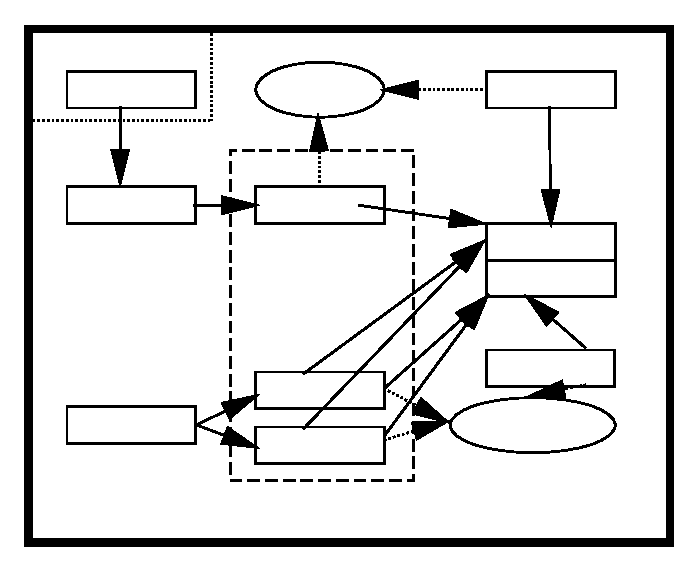
\includegraphics{sercom_handshake}}
    \put(117.44,49.67){\fontsize{7.07}{8.48}\selectfont BinaryModeRead(..)}
    \put(117.44,76.07){\fontsize{7.07}{8.48}\selectfont TextModeRead(..)}
    \put(127.02,220.54){\fontsize{8.83}{10.60}\selectfont notSent}
    \put(225.68,59.49){\fontsize{8.83}{10.60}\selectfont hshake\symbol{95}sent}
    \put(108.63,115.68){\fontsize{5.30}{6.36}\selectfont These methods work with Serial Port.}
    \put(26.79,59.35){\fontsize{8.83}{10.60}\selectfont Read(..)}
    \put(117.44,164.96){\fontsize{8.83}{10.60}\selectfont AsyncSend(..)}
    \put(26.79,164.96){\fontsize{8.83}{10.60}\selectfont Send(..)}
    \put(228.32,147.36){\fontsize{8.83}{10.60}\selectfont CallKof(..)}
    \put(228.32,129.76){\fontsize{8.83}{10.60}\selectfont CallOkf(..)}
    \put(228.14,86.63){\fontsize{8.83}{10.60}\selectfont CheckSD(..)}
    \put(228.32,220.40){\fontsize{8.83}{10.60}\selectfont CheckNS(..)}
    \put(26.79,220.40){\fontsize{8.83}{10.60}\selectfont public Write(..)}
    \end{picture}%
  \fi
  \caption{\label{pic:sercom_handshake}%
   Sercom current design}
  \end{figure}

  The answers of $Sercom$ are processed in the $Read$ function
  which is the $DataReceived$ handler of .Net $SerialPort$. The $DataReceived$ handler is called asynchronously
  in .Net implementation of the $SerialPort$ class if at least one new character is deliver to
  serial port input buffer. 

  The $Read$ method which is called asynchronously just calls $textModeCall$
  in the text mode and $binaryModeRead$ in the binary mode.
  The only command, which is sent in the binary mode in {\it Elib}, is the command to get a picture.
  The picture is the only binary answer of {\it BTCom} too.
  A description of $binaryModeRead$ is postponed after  
  a introduction $textModeCall$ method.
  
  Every time the $textModeCall$ is raised, the new characters are step by step
  added to the $ans$ container. If the whole answer is stored in $ans$, $ans$ is cleared.
  The found $answer$ is checked against $ansGuard$ stored in $hshake\_sent$.
  If it matches, the $Okf$ callback is called and the $hshake\_sent$ variable is set to $null$. 
  Also the $Send$ function is called via the $Received$ delegate. If the answer does not match, it is thrown away. 
  
  If the binary mode is on, the $binaryModeRead$ procedure is called from
  the $Read$ function. The $binaryModeRead$ does not read bytes step by step.
  At first it reads first three bytes where width, height and mode of a picture is stored.
  The total size of a picture is computed from the first three bytes of the picture.
  After receiving the first three bytes the function tries to read remaining bytes.
  The bytes are usually transferred split into several parts,
  because the reading is performed in separate thread and 
  the operating system switch to different thread during the reading.
  If the picture is transferred before the $timeout$ elapsed, then the $Okf$ callback is called.
  The $Kof$ callback is called otherwise. 
  If $Sercom$ is receiving the picture and the timeout elapses,
  $Sercom$ continues receiving the picture. $Sercom$ stops the receiving only if
  the image is complete or if no bytes have been received longer than 0.1 seconds.
  The $Kof$ callback of "GetImage" command is the only $Kof$ callback 
  that can have the answer at disposal, so the picture is passed to $Kof$ callback too.	
  After $Kof$ or $Okf$ call in binary mode instance of $ansGuard$ is removed from $hshake\_sent$ 
  and $Send$ method is invoked using $Received$ event.
  The last action of $binaryModeRead$ is to switch the flag from binary mode to text mode.
  
  The {\it BTCom} switches back to the text mode automatically, because
  the "GetImage" command is sent in binary mode to e-Puck together with an empty byte, which
  switches {\it BTCom} on e-Puck  immediately after sending the picture back to the text mode.

  Sending and receiving commands replies works well 
  until an answer is lost. $Timeouts$ ensure that the stacked instance of $ansGuard$ are cleared after its $timeout$  elapses.
  The instance of $ansGuard$ is stacked either in $notSent$ queue	or in $hshake\_sented$.
  Both methods, which implement the removal of an $ansGuard$, run in worker threads and also implement
  sophisticated system of waking and putting their threads to sleep, which prevents the threads from wasting
  the CPU time during their waiting to the $timeout$ expiration. 
  The $checkSD$ function looks after the $ansGuard$ in $hshake\_sent$ and the $checkNS$ function guards
  the $ansGuards$ in the $notSent$ queue.

  Putting the functions into sleep is complicated, because the $ansGuard$ has to be moved or deleted thread-safely,
  which means synchronization primitives has to be used multiple times.
  
  %todoooooo todo todddddddddddddddddddddooo vysvetlit proc pri atomizovani se to muze zablokovat a proc jsou 
  %potreba dva EventWaitHandle
  
  $Sercom's$ inner structure have been depicted. For details of 
  $Sercom$ implementation see the code and the reference documentation in enclosed CD.

  Let  us present the interface of $Sercom$ and its public members.
  Figure \ref{publicser} lists all public functions of $Sercom$.
  The $Write$ function has been already introduced. The $Write$ function can be used only
  after the $Start$ function is called. The $Start$ function is called only once and
  it opens serial port and initialise the {\it BTCom} communication. 
  The serial port is opened with parameters set in the constructor of $Sercom$ or with
  default parameters specified in $Sercom$ in $Sercom's$ constants. The $Dispose$ method closes the serial port
  and prepares $Sercom$ for a garbage collection.

\begin{figure}[!hbp]
\begin{lstlisting}[language=cs]
public class Sercom:IDisposable{
  public void Write(string command, RCallback okf, NRCallback kof,object state, double timeout);
  public void Start();
  public Sercom(string portName, int serialPortWriteTimeout, int serialPortReadTimeout);
  public Sercom(string portName) : //with default constants
        this(portName, defWriteTimeout, defReadTimeout) { }
  public int NotAnswered{get;}
  public int NotSent{get;}
  public byte[] LastImgBytes{get;}
  public bool FullImgBytes{get:}
  public int ModeImg{public get:}
  public int HeightImg{public get;}
  public int WidthImg{public get;}
  public void Dispose();
}
\end{lstlisting}
\caption{Public functions of $Sercom$} \label{publicser}	
\end{figure}

  There are also several properties available. The $NotAnswered$ and $NotSent$ properties
  show how much is the instance $Sercom$ class occupied. $NotSent$ returns only the length of the $notSent$ queue. 
  $NotAnswered$ is at most by one greater than $NotSent$,
  because it returns number of $ansGuards$ in $notSent$ plus one if is an $ansGuard$ in $hshake\_sent$.

  The remaining properties are attributes of the last taken image. They are valid, if the $FullImgBytes$ is set to true.
  Otherwise the properties are not all from the last image.
  If the $Okf$ was called on the last taken image then $FullImgBytes$ is always set to $true$. The property
  comes in use if the $Kof$ callback was called, because it can be called from $notSent$ queue 
  or the bytes of image got lost, or the image is all right, but it was received too late. 
  From width, height, mode and bytes a bitmap can be built, which is perfromed
  in the $Epuck$ class.

\section{The $Epuck$ class} \label{sec:epuck}
  An instance of $Epuck$ offers a virtual representation of e-Puck,
  which intermediates all sensors and actuators of e-Puck to user. 
  The $Epuck$ class also hides Bluetooth communication from the user.

  $Epuck$ uses $Sercom$ internally and makes controlling of robot much more comfortable.
  $Sercom$ treats only the command "GetImage" specially, because it is the only one command in binary mode
  and it has big time requirements. $Sercom$ does not differentiates between other commands.
  $Epuck$ differentiate between commands a lot. It tights $Epuck$ with concrete implementation of {\it BTCom},
  but it also allows to process the answers and to offer a typing of the returning values, which increases
  applicability. Main goal of the $Epuck$ class is to offer a good interface.

  In this chapter the usage of $Sercom$ in $Epuck's$ class is presented together with additional methods 
  for implementation of the interfaces. The reasons, which lead to implementing two independent interfaces for
  controlling e-Puck robot through $Epuck$ class, are presented.
  Last but not the least the used technology of .Net is mentioned.

  The $Epuck$ class brings nothing more than interface and debugging tools. We describe the interface
  on examples as much as possible. There are several introductory examples in these chapter,
  which explain the properties of the interface. Furthermore, 
  Guide lines for the $Epuck$ class and the debugging
  tools can be found in Chapter ~\ref{chap:usage}.
  The following sections present the internals of $Epuck's$ methods.
  
\subsection{Typed functions with $Okf$ and $Kof$ callbacks} \label{sec:okfkofi}
  $Epuck's$ basic interface just wraps the $Sercom$ class. It differentiates between
  commands for actuators, sensors with string return value and sensors, which return an array of integers.
  $Epuck$ treats pictures differently too, because it passes to callback a $Bitmap$ instance.


\begin{figure}[!hbp]
\begin{lstlisting}[language=cs]
public class Epuck{
  public void Stop(OkfActuators okf, NRCallback kof, object state, double timeout) {
          actuators(Commands.c_Stop(),okf,kof, state, timeout, "Stop(..)");
  }
  public void GetIR(IntSensorsOk okf, NRCallback kof, object state, double timeout) {
          IntArrSensors(Commands.c_Proximity(),8,okf,kof,state,timeout,"GetIR(..)");
  }
  public void GetBTComVersion(stringSensors(..)Ok okf, NRCallback kof, object state, double timeout) {
          stringSensors(..)(Commands.c_Version(), okf, kof, state, timeout, "BTComVersion(..)");
  }
  public void GetPicture(CamSensor okf, CamSensor kof, object state, double timeout) {
          checkArgs(okf, kof, timeout);
          logf(Action.call, f_name);
          ser.Write(Commands.c_GetImage(),
          (ans, data) => {
            okf(parsingBitmap(ser.LastImgBytes, ser.WidthImg, ser.HeightImg, ser.ModeImg), data);
            logf(Action.ok, f_name);
          },
          (data) => {
            if (ser.FullImgBytes)//a whole img was captured
              kof(parsingBitmap(ser.LastImgBytes, ser.WidthImg, ser.HeightImg, ser.ModeImg), data);
            else
              kof(null, data);//img is demaged
            logf(Action.ko, fname);
          },
          state,timeout);		
  }	   
}
\end{lstlisting}
\caption{Four types of $Epuck$ control functions}
\label{publicep}	
\end{figure}

  Although there are four kinds of commands, the implementation differs only in processing the answer.
  The processing functions $actuators(..)$, $intArrSensors(..)$, $stringSensors(..)$ all 
  look like $GetImage(..)$ method.
  
  There are only two differences between $GetImage(..)$ and other functions.
  Other functions have to parse the answer in $Okf(..)$ functions differently and they do not parse
  answer in $Kof(..)$ callback at all.

  $GetImage(..)$ calls on answer $processBitmap(..)$.
  The function $actuators(..)$ throws away the string answer, because the answer contains no useful information.
  The $stringSensors(..)$ method just calls $Okf(..)$ with the string answer.
  $IntArrSensors(..)$ parse the string answer and calls $Okf(..)$ with an $int$ array argument.

  The second difference is that $Kof(..)$ function from $GetPicture(..)$ gets the answer. 
  Other $Kof(..)$ callbacks have only one parameter $state$, 
  because there is no answer available at the moment of calling $Kof(..)$.
  See ~\ref{p:oneargument} for more information.

  The differences between $GetImage(..)$ and the processing functions are expressed by use of different
  delegates for $Okf(..)$ functions. All $Kof(..)$ functions fits to same delegate $KofCallback$. 
  Only the $GetImage(..)$ function defines its own delegate $OkfKofCamsSensor$, 
  which $GetImage(..)$ also uses for the $Okf(..)$ functions.

  As you can see in Figure ~\ref{publicep}, the callbacks are wrapped in lambda functions \cite{lambda}
  instead of passing $Okf(..)$ and $Kof(..)$ directly to $Sercom.Write(..)$ function.
  $Okf(..)$ and $Kof(..)$  are called within the lambda functions.
  The lambda functions allow logging and parsing the answers.

  A function $checkArgs$ at the beginning of $GetPicture(..)$ does not allow to pass invalid arguments
  to $Epuck$ functions. $Timeout$ has to be a positive $double$ value, $Okf$ and $Kof$ delegates 
  has to be defined and not set to $null$.

  $Okf(..)$ callbacks should be used for implementing the desired algorithm by an {\it Elib} user.
  On the other hand, $Kof(..)$ callbacks should perform repair actions in order to get into a valid state,
  where the algorithm can be restarted. A programmer, which uses {\it Elib} should always have in mind,
  that $Kof(..)$ callbacks can be raised very often for low $timeouts$,
  but the call of $Kof(..)$ callback signalizes a serious error state.
  See Section ~\ref{sec:interfaces} for more examples of how to use $Okf(..)$ and $Kof(..)$ callbacks.


\subsection{The $IAsyncResult$ interface} \label{sec:iasync}
  Two callbacks and a schizophrenic logic of the $Okf(..)$ and $Kof(..)$ implementation are not
  convenient for exploring e-Puck's sensors and actuators, 
  however they allow e-Puck to easily recover from every situation.

\begin{figure}[!hbp]
\begin{lstlisting}[language=cs]
interface IAsyncResult{
  public Object AsyncState { get; }
  public Boolean CompletedSynchronously{get; } 
  public WaitHandle AsyncWaitHandle { get; }
  public Boolean IsCompleted { get; }
}
\end{lstlisting}
\caption{$IAsyncResult$ interface}
\label{interface}
\end{figure}

  Motivation for implementing the $IAsyncResult$ is its clear usage and its proven usability.
  See Chapter ~\ref{chap:usage} for $IAsyncResult$ introduction and examples.
  The requirements of interface is shown in Figure ~\ref{interface}

  The $IAsyncResult$ is introduced in Figure ~\ref{arexample}, which uses $ada$ instance
  of $Epuck$ to get IR sensor values from a real e-Puck. The $timeout$ is the only parameter of $BeginGetIR(..)$,
  which has nothing to do with $IAsyncResult$ interface.

\begin{figure}[!hbp]
\begin{lstlisting}[language=cs]
IAsyncResult ar = ada.BeginGetIR(timeout, callback, state);            
int[] IRSensors = ada.EndGetFtion(ar); //if callback == null
\end{lstlisting}
\caption{Usage of $IAsyncResult$}\label{arexample}
\end{figure}

  An asynchronous operation implemented by $IAsyncResult$ needs two functions. The first function usually starts with 
  "$Begin$" prefix and the second starts with "$End$" prefix. This convention is strictly respected in {\it Elib}.
  $BeginGetIR(..)$ is example of the first function and $EndGetFtion(..)$ of the second function.
  $BeginGetIR(..)$ takes three arguments. 

  If the $callback$ delegate is null, then we need the $EndGetFtion(ar)$ function
  in order to be sure that the real e-Puck has sent the values of IR sensors. 
  See the Figure ~\ref{arexample}.
  The call of $EndGetFtion(..)$ blocks the current thread and waits synchronously until the real
  e-Puck is stopped.

  If the $callback$ functions are defined, they are raised after the $BeginGetIR(..)$ function has finished.
  Usually, if $callback$ delegate is used, then the $EndFtion(..)$ function call is not necessary.

  The only possibility of $IAsyncResult$ interface to signal an error is raising an exception.
  The exception is passed to callback or the "End" function raises it.

  The $ar$ instance of $IAsyncResult$ allows the $EndGetFtion(..)$ to wait to the end of $BeginGetIR(..)$ function.
  The instance is also used for passing user defined data in $state$ object to the callback function,
  because $ar$ instance has a $ar.AsyncState$ reference to $state$ object.
  Another important feature of $ar$ is, that it allows $EndGetFtion$ function to receive the data
  from $ar$. For example an integer array of IR sensors' values can be extracted from $ar$ like in Figure ~\ref{arexample}.
  
  $IAsyncResult$ is widely used through .Net, but it is an asynchronous programming model
  and is a bit tricky in some situation. See various examples in Chapter ~\ref{chap:usage} 
  to get used to it.

\subsection{$IAsyncResult$ implementation} \label{sec:iasyncimpl}
  Jeffrey Richter \cite{IAsync} made a nice example of two classes, which implement $IAsyncResult$ interface.
  I used his classes and modified them according to {\it Elib}'s needs.
  The first class is $AsyncNoResult$ and implements $IAsyncResult$ for actuators.
  The second class is generic $AsyncResult<T>$ subclass of $AsyncNoResult$ and 
  it implements $IAsyncResult$ interface for sensors.
  Generic class mean, that the type of the result is chosen at compile time. %todo find definition
  Instances of $AsyncResult<T>$ are used
  for $String$, $Bitmap$ as well as integer array answers with a different generic parameter $T$.
  
  The idea of the $IAsyncResult$ interface is that a programmer does not have to know which
  class implements the $IAsyncResult$. They use $IAsyncResult$ type in a code. See Figure ~\ref{arexample}. 
  On the other hand, the functions $BeginGetIR$ and $EndGetFtion$ have to know the type, which is passed to $IAsyncResult$ object.
  "Begin" function in {\it Elib} creates the instances $AsyncNoResult$ for actuators and $AsyncResults<T>$ for sensors.
  "End" function in {\it Elib} waits until the end of "Begin" function and 
  throws an exception if the command has not been delivered in time.
  If the answer is delivered in time and if the command has requested a sensor value, 
  the "End" function returns the desired sensor's values.
  
\subsection*{Obligatory members of $IAsyncResult$} \label{sec:iasyncmemb}
  Let us examine in detail the $IAsyncResult$ interface from Figure ~\ref{interface}. 
  \begin{itemize}
  \item $AsyncState$ is an object used as argument for a callback function, which
  is passed to "Begin" function. If no callback is passed, the $AsyncState$ is not used. 
  $AsyncState$ is useful for passing information to the callback.
  \item $AsyncWaitHandle$ is a synchronisation primitive which allows waiting until the operation 
  started in "Begin" function is done.
  $AsyncWaitHandle$ is used in "End" function if the "End" function is called 
  and the operation is still running. 
  \item Flag $CompletedSynchronously$ tells whether  
  $AsyncWaitHandle$ has been used to wait to the end of the operation.
  $CompletedSynchronously$ is always set to false if callback is used.
  \item $IsCompleted$ tells whether the operation from "Begin" function terminated or not.
  \end{itemize}

\subsection*{The "Begin" and "End" functions} \label{sec:beginend}
  Let us describe public methods of $AsyncNoResult$, which are used to implement "Begin" and "End" functions.
  $IAsyncResult's$ properties are not enough to implement $BeginGetIR$,
  $EndGetFtion$ or any other "Begin" and "End" functions.
  $BeginGetIR$ method use a constructor of $AsyncNoResult$. It also uses the $SetAsCompleted$ function 
  and the $EndInvoke$ function both from $AsyncResult$ subclass.
  We will explain the interesting and crucial part of both classes. 
  For implementation details see code in Figure ~\ref{result} and ~\ref{noresult}.

  A constructor of $AsyncNoResult$ only sets the field members, 
  which are not changing during $AsyncNoResult$ existence.
  The implementation of $SetAsCompleted(..)$ method from $AsyncNoResult$ sets an exception to $AsyncNoResult$.
  $SetAsCompleted(..)$ from $AsyncResult$ overloads $SetAsCompleted(..)$ method
  from its base class $AsyncNoResult$ and adds a possibility to set the results instead of the exception.
  Third overload is implemented in $AsyncResult$ in order to the $GetPicture(..)$ command can set both 
  exception and the result at one time.
  $EndInvoke(..)$ is called from "End" function and does all its logic. It checks whether the called 
  operation has finished.	If the operation is still pending, it sets up a new $AsyncWaitHandle$
  and waits to its termination. At the end it throws an exception if one has been set up, 
  or it returns a result if $EndInvoke(..)$ from $AsyncResult$ was called.

\begin{figure}[!hbp]	
\begin{lstlisting}[language=cs]
public class AsyncResultNoResult : IAsyncResult {
  // Fields set at construction which never change 
  readonly AsyncCallback m_AsyncCallback;
  readonly Object m_AsyncState;
  // Fields which do change after operation completes
  const Int32 c_sp = 0;//StatePending
  const Int32 c_scs= 1;// StateCompletedSynchronously
  const Int32 c_sca = 2;//StateCompletedAsynchronously
  Int32 m_CompletedState = c_sp;
  // Field that may or may not get set depending on usage
  ManualResetEvent m_AsyncWaitHandle;
  // Fields set when operation completes
  Exception m_exception;
  // Name makes debugging easier in Elib. It shows, which command was used.
  string name;
  public string Name { 
          get { return (name != null) ? name : ""; } 
          set { name = value; 		} 
  }
  public AsyncResultNoResult(AsyncCallback asyncCallback, Object state, string name_) {
          m_AsyncCallback = asyncCallback;
          m_AsyncState = state;
          name = name_;
  }
  public AsyncResultNoResult(AsyncCallback asyncCallback, Object state) : 
          this(asyncCallback, state, null) { }
  public void SetAsCompleted(Exception exception, Boolean completedSynchronously) {
          // Passing null for exception means no error occurred. 
          // This is the common case
          m_exception = exception;
          // The m_CompletedState field MUST be set prior calling the callback
          Int32 prevState = Interlocked.Exchange(ref m_CompletedState, 
                  completedSynchronously ? c_scs : c_sca);
          if (prevState != c_sp)
                  throw new InvalidOperationException("You can set a result only once");
          // If the event exists, set it
          if (m_AsyncWaitHandle != null) m_AsyncWaitHandle.Set();
          // If a callback method was set, call it
          if (m_AsyncCallback != null) m_AsyncCallback(this);
  }
  public void EndInvoke() {
          // This method assumes that only 1 thread calls EndInvoke 
          // for this object
          if (!IsCompleted) {
                  // If the operation isn't done, wait for it
                  AsyncWaitHandle.WaitOne();
                  AsyncWaitHandle.Close();
                  m_AsyncWaitHandle = null;  // Allow early GC
          }      
          // Operation is done: if an exception occured, throw it
          if (m_exception != null) throw m_exception;
  }

  //region Implementation of IAsyncResult
  public Object AsyncState { get { return m_AsyncState; } }
  public Boolean CompletedSynchronously{get { 
          return Thread.VolatileRead(ref m_CompletedState) ==  ic_scs; }}
  public WaitHandle AsyncWaitHandle {
      get {
          if (m_AsyncWaitHandle == null) {
            Boolean done = IsCompleted;
            ManualResetEvent mre = new ManualResetEvent(done);
            if (Interlocked.CompareExchange(ref m_AsyncWaitHandle,
               mre, null) != null) {
              // Another thread created this object's event; dispose 
              // the event we just created
              mre.Close();
            } else {
              if (!done && IsCompleted) {
                // If the operation wasn't done when we created 
                // the event but now it is done, set the event
                m_AsyncWaitHandle.Set();
              }
            }
          }
          return m_AsyncWaitHandle;
      }
  }
  public Boolean IsCompleted {
          get {return Thread.VolatileRead(ref m_CompletedState) != c_sp; }}
  //endregion Implementation of IAsyncResult
}
\end{lstlisting}
\caption{$AsyncNoResult$} 
\label{noresult}
\end{figure}


  An interesting feature of $AsyncNoResult$ which is inherited by $AsyncResult$ is a creation of an $EventWaitHandle's$ instance.
  It is not created in all cases and is created at most one in a $AsyncNoResult's$ life cycle.
  An instance of $EventWaintHandle$ is created only if the user explicitly called get method for $WaitHandle$ or
  if the $EndInvoke$ method was called and the operation is still pending.
  It means that if you use callback and do not call "End" function then no instance of $EventWaitHandle$ is created.
  Let us stress that $EventWaitHandle$ is provided from an operating system and its instantiation is relatively slow.

  The $name$ field seems useless, but it allows "Begin" function to put its name in it. 
  The name can be used in logging or debugging, which will be described in following paragraphs devoted 
  to design of "Begin" and "End" functions.

  Let us note that $AsyncResutl$ adds no crucial logic except setting a result in $SetAsCompleted$ function and
  returning the result in $EndInvoke$ function. 
  $AsyncResult$ use its base class $AsyncNoResult$ to implement the logic.
\begin{figure}[!hbp]
\begin{lstlisting}
public class AsyncResult<TResult> : AsyncResultNoResult {
  // Field set when operation completes
  TResult m_result = default(TResult);
  public AsyncResult(AsyncCallback asyncCallback, Object state,string name) : 
    base(asyncCallback, state,name) { }
  public AsyncResult(AsyncCallback asyncCallback, Object state) : 
    this(asyncCallback, state, null) { }
  //enable to set Result. AsyncNoResult enables to set exception.
  public void SetAsCompleted(TResult result, Boolean completedSynchronously) {
    // Save the asynchronous operation's result
    m_result = result;
    // Tell the base class that the operation completed 
    // sucessfully (no exception)
    base.SetAsCompleted(null, completedSynchronously);
  }
  // Allows to set both the exception and the result. Added for GetImage(..).
  public void SetAsCompleted(TResult result, Boolean completedSynchronously, Exception exception) {
    m_result = result;
    base.SetAsCompleted(exception, completedSynchronously);
  }
  new public TResult EndInvoke() {
    base.EndInvoke();// Wait until operation has completed 
    return m_result; // Return the result (if above didn't throw)
  }
}
\end{lstlisting}
\caption{$AsyncResult<T>$} \label{result}
\end{figure}

  Let us introduce an implementation of "Begin" and "End functions.
  They are the tools for manipulating e-Puck easily and they are the key functions of the $IAsyncResult$ implementation.
  All the "Begin" and "End" functions' implementations are similar. The implementations look like $BeginGetIR's$
  and $EndGetFtion's$ implementations from ~\ref{arexample}.
  The implementation of $BeginGetIR's$ and its "End" function is shown in Figure ~\ref{beginsens}.
  All "Begin" functions use $Epuck's$ interface with the $Okf$ and $Kof$ callbacks introduced
  in Subsection ~\ref{sec:approach}.	

\begin{figure}[!hbp]
\begin{lstlisting}
public IAsyncResult BeginGetIR(double timeout, AsyncCallback callback, object state) {
  AsyncResult<int[]> a = 
  new AsyncResult<int[]>(callback, state, logFunctionNames["BeginGetIR(..)"]);
  GetMikes(receivedSensors<int[]>, failed, a, timeout);
  return a;
}
static T EndSensors<T>(IAsyncResult ar) {
  AsyncResult<T> a = (AsyncResult<T>)ar;
  return a.EndInvoke();
}
public int[] EndGetFtion(IAsyncResult ar) { 
  return EndSensors<int[]>(ar); 
}
\end{lstlisting}	
\caption{An example of "Begin" and "End" function for sensors.}
\label{beginsens}
\end{figure}

  The "Begin" function creates an $AsyncNoResult$ respectively $AsyncResult$ instance called $a$. 
  The function pass the supplied callback with its $state$ object to
  $a$. Third argument of $a's$ constructor is a name of the used function.
  $BeginGetIR(..)$ instantiate $AsyncResult<int[]>$, because $BeginGetIR(..)$
  expect array of $ints$ as its answer. 
  The $Name$ field of $AsyncResult$ is filled with the $string$ value from $logFunctionNames$ dictionary. 
  The dictionary values are by default set to their key values, so
  the $Name$ in $BeginGetIR(..)$ function is filled with "BeginGetIR(..)" value.
  After setting up the $a$ instance the $GetMikes(..)$ function is called with the $receiveSensors<int[]>(..)$ and 
  $failed(..)$ methods as $Okf(..)$ and $Kof(..)$ callbacks.
  The $a$ instance is passed as the $state$ argument and is at disposal to the $failed(..)$ and 
  $receiveSensors(..)$ functions.
  The function $receiveSensors(..)$ is called with generic parameter $int[]$, 
  because the $GetIR$ values expect an array of $ints$ from sensor.
  The function, which control actuators, calls the $received(..)$ function as the $Okf(..)$ callback. 
  See an example in Figure ~\ref{beginact}.
  Sensor's methods as well as actuator's methods use the $failed(..)$ function as its $Kof(..)$ callback.
  An exception is the $GetImg(..)$ function which uses the $failedBitmap(..)$ callback instead.
  The last action of each "Begin" function is a return of the instance $a$.

  Let us shortly introduce the "End" functions before we will focus on the $Okf(..)$ and 
  $Kof(..)$ callbacks used in the "Begin" functions.
  There are two tasks of the "End" functions.
  The first task  is to cast the $IAsyncResult$ argument to the correct type of $AsyncResult$ 
  or to the $AsyncNoResult$ class. The second task is to call the $EndInvoke(..)$ method.
  If the "End" function is called with an $IAsyncResult$ argument from a sensor command, 
  the value from $EndInvoke(..)$ is returned. See Figure ~\ref{beginsens}. 
  If the $IAsyncResult$ argument is passed from the "Begin" function, 
  which controls an actuator, then $EndInvoke(..)$ is called and nothing is returned. See Figure ~\ref{beginact}.
  
\begin{figure}[!hbp]
\begin{lstlisting}
public IAsyncResult BeginMotors(double leftMotor, double rightMotor, 
double timeout, AsyncCallback callback,Object state) {
AsyncResultNoResult a = 
new AsyncResultNoResult(callback, state,logFunctionNames["BeginMotors(..)"]);
Motors(leftMotor, rightMotor, received, failed, a, timeout);
return a;
}
public void EndActuators(IAsyncResult ar) {
AsyncResultNoResult a = (AsyncResultNoResult)ar;
a.EndInvoke();
}
\end{lstlisting}	
\caption{An example of "Begin" and "End" function for actuators.} \label{beginact}
\end{figure}
  
  The callbacks are called after the delivery of the answer or after the $timeout$ expiration.
  The callback allows to process the result of the operation.
  In the $IAsyncResult$ interface the results are set via calling the $SetAsCompleted$ method 
  on the $AsyncNoResult$ respectively $AsyncResult$ instance.
  If the operation fails, the $Kof$ callback $failed$ is called. 
  In the $failed$ function the $SetAsCompleted$ method is called and an exception is passed to first argument $SetAsCompleted$.
  See the first function $failed$ in Figure ~\ref{Ikofs}.

  The only exception that can return both the exception and the result is the $BeginGetPicture(..)$ function.
  The function $receivedSensors<Bitmap>$ is used in the $Okf$ delegate $BeginGetPicture(..)$, and 
  the special function $failedBitmap(..)$ is called if an exception has been raised.
  The $Kof(..)$ callback raise a special exception, if the image was captured and has been 
  delivered after timeout expiration.
  Implementation is shown in Figure ~\ref{Ikofs}. 

  
\begin{figure}[!hbp]
\begin{lstlisting}
static void failed(object asyncNoResult) {
  AsyncResultNoResult ar = (AsyncResultNoResult)asyncNoResult;
  ar.SetAsCompleted(new ElibException(ar.Name + " command hasn't been confirmed in timeout"), false); 
}
static void failedBitmap(Bitmap pic,object asyncResult) {
  if (pic != null) {
    AsyncResult<Bitmap> ar = (AsyncResult<Bitmap>)asyncResult;        
    ar.SetAsCompleted(pic, false, new ElibException(ar.Name + 
      " command GetPicture has not been confirmed in timeout, but picture is still available in AsyncResult<Bitmap>"));
  } else
    failed(asyncResult);
}
\end{lstlisting}	
\caption{$Kof$ callbacks for $IAsyncResult$} \label{Ikofs}
\end{figure}


  If the answer is delivered in time, then the $Okf$ callback is called.
  The sensor's callback $receivedSensors<T>$ passes the answer of the type $T$ to its first argument.
  The actuators callback $received$ just passes $null$ to its first argument, which indicates
  raising of no exception.
  See the code below in Figure ~\ref{Iokfs}.


\begin{figure}[!hbp]
\begin{lstlisting}
static void received(object asyncNoResult) {
  AsyncResultNoResult ar = (AsyncResultNoResult)asyncNoResult; ar.SetAsCompleted(null, false); 
}
static void receivedSensors<T>(T b, object asyncResIntArr) {
  AsyncResult<T> a = (AsyncResult<T>)asyncResIntArr;
  a.SetAsCompleted(b, false);
}
\end{lstlisting}	
\caption{$Okf$ callbacks for $IAsyncResult$} \label{Iokfs}
\end{figure}

\section{Summary of Elib interfaces}
\label{sec:suminterface}
  In previous three subsections the implementations of the two interfaces of $Epuck$ 
  and one $Sercom's$ interface have been described.

  $IAsyncResult$ is built on the basic $Epuck's$ interface with the typed $Okf(..)$ and $Kof(..)$ callbacks. 
  The basic $Epuck$ interface is itself built on $Sercom's$ $Okf$ / $Kof$ interface.
  The purpose of the interfaces is to make programming e-Puck over Bluetooth easier.
  The $IAsyncResult$ is the most comfortable of the three interfaces. 
  The use of $Sercom's$ interface needs good knowledge of BTCom protocol and 
  it forces user to process every answer of {\it BTCom}.

  Let us compare the possibilities and limitations of the interfaces against each other.
  The $Sercom's$ interface and $Epuck$ basic interface with $Okf$ and $Kof$ 
  have the same limitations and possibilities for the e-Puck running {\it BTCom} version 1.1.3. 
  
  Every program written using $Epuck's$ basic interface can be written
  in $Sercom$ by implementing $Epuck's$ interface as it is in {\it Elib}.
  On the other hand, every program, which uses $Sercom$ interface and communicates with {\it BTCom}
  version 1.1.3 on e-Puck, can be written using $Epuck's$ basic interface. 
  $Epuck's$ basic interface is a specialization of $Sercom$ for concrete version of {\it BTCom}
  protocol.

%%%%todo vyjasnit a vysvetlit, ze jde simulovat kof pomoci IAsyncResult
  $IAsyncResult$ limits the role of the $Kof$ callback, but does not limit the role of the $Okf(..)$ callback.
  If a user wants to implement an $Okf$ logic using the $IAsyncResult$ interface, he uses callback from $IAsyncResult$
  interface, which is passed to the "Begin" function.
  The callback is called after the $received$ respectively $receivedSensor<T>(..)$ function  call 
  the $SetAsCompleted(..)$ method on an $a$ instance of $IAsyncResult$. 
  Remind the implementation in Figure ~\ref{Iokfs}.
  The $received(..)$ and $receivedSensor<T>(..)$ functions are called as the $Okf$ callbacks
  from the $Epuck's$ basic interface.
  See Figure ~\ref{beginact} and Figure ~\ref{beginsens} for the confirmation.
  To conclude the $IAsyncResult$ callback is invoked in the $Okf(..)$ callback of $Epuck's$ basic interface.

\begin{figure}[!hbp]
\begin{lstlisting}
static void SimulatingKof_over_IAsResult(Epuck ada) {
  //the timeout is too small!
  ada.BeginGetImage(0.001, okf, ada);
}
\end{lstlisting}
\caption{Start of the behaviour.}
\label{c:start}
\end{figure}

  The limitation of $IAsyncResult$ arises from setting an exception in the $Kof(..)$ callbacks,
  which are used in the $IAsyncResult's$ implementation.
  On the other hand, the functions in Figures ~\ref{c:start} and ~\ref{c:okfsim} use the $kof(..)$ callback function
  from Figure ~\ref{iasynckof} 
  which implements the $Kof$ logic in spite of the functions use $IAsyncResult$ interface.

  The $Kof$ logic should be implemented if an exception is raised. 
  The exception is raised in callback passed to $IAsyncResult$ if the answer is not delivered in timeout. 
  The nearest place, where it can be caught is in the call of the $EndInvoke$ method.
  The called $EndInvoke$ method is associated with the $IAsyncResult$ instance. 
  The common way for a user to invoke the $EndInvoke$ method is to call the "End" method 
  on the instance of $Epuck$ with the $IAsyncResult$ object as its parameter. 
  This technique is used in Figure ~\ref{c:okfsim}.
  The call of $ada.EngGetImage(ar\_)$ gets the image and the callback function continues
  or the $EndGetImage(..)$ function throws an exception which is caught by $try-catch$ block.
  In $catch$ block the user defined $kof$ function is invoked.
  
\begin{figure}[!hbp]
\begin{lstlisting}
//It can be only a callback of BeginGetImage,
//because the ar paramater has to contain a Bitmap
//See 8. row!
static void okf(IAsyncResult ar_) {
  if (!endf) {
    Epuck ada = (Epuck)ar_.AsyncState;
    try{
      Bitmap b = ada.EndGetImage(ar_);//no EventWaitHandle created
      IAsyncResult ar = ada.BeginMotors(-1, 1, 0.1, null, null);// some work
      //simulate image processig
      Thread.Sleep(20);
      ada.EndFtion(ar);
      //the timeout is too small!
      ada.BeginGetImage(0.01, okf, ada);
    } catch (ElibException) {
      //has to be fixed in kof
      ada.BeginStop(0.1, kof, ada);
    }
  } else
    endconfirmed.Set();
}
\end{lstlisting}
\caption{The $Okf$ callback with too small timeout.}
\label{c:okfsim}
\end{figure}

  The logic of the $Kof(..)$ function from the basic $Epuck's$ interface is preserved, because the user-defined
  $kof(..)$ is called in the same case when the $Kof(..)$ is called. Both are invoked if the $timeout$ expires.
  On the other hand, the $kof(..)$ uses an extra command to be invoked. In Figure ~\ref{c:okfsim} it
  is $ada.BeginStop(..)$ command, which invokes $okf(..)$. The $Stop(..)$ function would be the first command
  in $Kof(..)$ logic implementation of $Epuck's$ basic interface.
  The second difference is that the same $Kof(..)$ callback is called from $EndGetImage(..)$ and from the
  commands in the body. In this example the same $kof(..)$ is called for $EndGetImage(..)$ and 
  for $EndActuators(..)$, which is the pair function of the $BeginMotors(..)$ 
  command from the body of the $okf(..)$ function.
  The exception's origin can be found out from the $message$ property of exception, 
  where the $Name$ property of the $AsyncNoResult$ instance is used.

  The unknown source of exception is as well as the extra invocation command a minor problem, because
  there is usually only one $Kof(..)$ callback that consists of more than one command. 
  The $Kof$ logic complicates the program, so it is necessary to keep it simple in $Epuck's$ basic interface.

  The lost answer usually completely breaks the logic of $Okf$ implementation.
  The appropriate solution is to put e-Puck
  at the starting position of the behaviour. Usually, commands to stop e-Puck are sent 
  and a message is sent to the user or to the logging file.
  See Figure ~\ref{iasynckof}.

\begin{figure}[!hbp]
\begin{lstlisting}
//It can be called from any function,
//because we call only EndFtion!
//It can be applied to every IAsyncResult in Elib.
//See 7. row!
static void kof(IAsyncResult ar_) {
  if (!endf) {
    Epuck ada = (Epuck)ar_.AsyncState;
    ada.EndFtion(ar_);
    try {
      IAsyncResult ar = ada.BeginStop(to, null, null);//do the repair actions
      ada.EndFtion(ar);
      Console.WriteLine("The problem is fixed. Lets call okf!");
      ada.BeginGetImage(0.1, okf, ada);
    } catch (ElibException) {
      ada.BeginStop(0.1, kof, ada);
    }
  } else
    endconfirmed.Set();
}
\end{lstlisting}
\caption{Simulation of $Kof$ using $IAsyncResult$}
\label{iasynckof}
\end{figure}

  We have concluded that the $Sercom$ interface, the $Epuck's$ basic interface and 
  the $IAsyncResult$ interface have equal power for implementing algorithms.
  Let us explore the demands and the load of operating system (OS) when we use these interfaces.
  The more sophisticated the interface is, the bigger demands on OS it has.
  It is a consequence of building one interface upon the other.
  Let us stress that every program written using $IAsyncResult$ interface, 
  can be written with less or equal system resources using $Sercom's$
  interface. On the other hand, the programmers, 
  who use more complicated interface, for example the $Sercom$ class, do not usually find better way 
  than the one that is designed by the richer interface like $IAsyncResult$.

  In fact, $IAsyncResult$ is not much more demanding than $Sercom$ interface, if it is not misused.
  The only field, where $IAsyncResult$ does not keep up with $Sercom's$ interface, 
  is an extremely frequent calling of $Kof$ callbacks.
  $IAsyncResult$ throw an exception for every $Kof$ callback invocation, 
  whereas $Sercom's$ interface just needs to invoke a callback.
  $IAsyncResult$ also needs to call other functions, but it is quite fast. 
  The raising and catching an exception is significantly slower.
  On the other hand, such behaviour that extensively uses $Kof$ callbacks 
  has very special purpose or is a bad programming style.
  See Chapter ~\ref{chap:usage} for guidelines how to use the interfaces.

  The only resource, which can be extensively used in $IAsyncResult$, is $EventWaitHandle$. 
  $EventWaitHadndle$ is a synchronisation primitive provided
  by OS. There is at most one $EventWaitHandle$ created for each instance of $IAsyncResult$ in {\it Elib}. 
  On the other hand, by using callbacks in {\it Elib's} $IAsyncResult$
  implementation, the creation of $EventWaitHandles$ is completely avoided.

  Let us note that $Sercom's$ and the simple $Epuck's$ interface 
  are almost identical and therefore they have almost identical performance.
  The $Epuck$ class adds answers processing and allows logging. The user would do the processing of the answers anyway.
  If the logging is off, the one additional "if statements" in method adds no overhead. 
  Choosing one interface before another in {\it Elib} does not significantly influence the performance of application.

  We have put {\it Elib} to some tests. Let us introduce the results.
  The size of compiled {\it Elib} library is less 50 KB.
  Using $IAsyncResult$ in "Bull" behaviour  {\it TestElib} consumes 8512 KB of memory.
  Compare it with a simple console application, which needs 4580 KB of memory, or with Google Chrome, 
  which consumes more than 30000 KB of memory.
  %todo reference
  During three performance tests on $SimulatingKof\_over\_IAsResult(..)$
  numbers of threads of the {\it TestElib} application do not exceed 10. 
  See Section ~\ref{iasynckof}. Moreover, the threads were usually unused
  in $ThreadPool$ system class which has used only one or two. 
  The two worker threads were running of course all the time.
   %csReadLineEmpty.exe 4580KB csReadLineEmpty.vshost.exe 15184KB
   %{\it TestElib }.vshost.exe consumed 14108KB

  The Table ~\ref{times1}  was measured using the $ConsoleTestSensorsTimeout$ and
  $ConsoleTestActuatorsTimeout$ functions with $timeout$ 10 seconds.
  It shows that most of commands are delivered under 0.1 seconds. 
  On contrary, the commands to take a picture or to set camera parameters, 
  which is very useful, last almost half a second. 
  The reason is that a camera is very demanding device and it produces a lot of data.
  The special commands for calibrating IR sensors and for reseting e-Puck lasted even longer.
  The "reset" command has even exceeded the $timeout$.

  The values in table were measured from 10 independent measurement. 
  The first six measurements used e-Puck with a not fully charged battery.
  The second test was performed on e-Puck with a recharged battery.

%1-3 neprazdna baterie debug
%4-6 not empty baterry, release 
%6-9 fully charge baterry, release 
%9-12 fully charge baterry, debug

\begin{table}[!hbp]
\begin{tabular}{lrrrrrr}
Command string & {\small Average (1. test)}  & {\small Variance (1. test)}& {\small Average (2. test)} & {\small Variance (2. test)}\\
GetHelpInfo(..)& 0.13873 & 0.00036& 0.12162&0.00007\\
GetAccelerometer(..)&0.07017&0.00009&  0.06393&0.00009\\ 
GetVersionInfo(..)&0.04153&0.00028&.05715&0.00055\\ 
GetCamParams(..)&0.04927&0.00001&  0.05073&0\\ 
GetEncoders(..)&0.0481&0.00012&  0.04015&0.00026\\ 
GetImage(..)&0.30715 &0.00118& 0.31232&0.00698\\ 
GetIR(..)&0.06543 &0.00011&0.05977&0.00008\\ 
GetIRInfo(..)&0.06002 &0.00055& 0.05053&0.00088\\
GetLight(..)&0.08305 &0.00083&0.0919&0.00106\\
Microphones(..)& 0.0319&0.00045 0.01868&0\\
ada.GetSelector(..)& 0.07517&0.00296& 0.04993& 0\\
GetSpeed(..)& 0.01298&0.00066&   0.00245&0.00001\\
Reset(..) &{\it 1.3942} & 0 &{\it 1.39023} &0.00007 \\
BodyLight(..)& 0.03253&0.00009&   0.03057&0.00004\\
CalibrateIRSensors(..)&3.69635&0.00006&3.69173&0.00013\\
FrontLight(..)&0.03123&0.00002 & 0.02998&0.00004\\
LightX(..)& 0.02515&0.00015&  0.02347&0.00012\\
Motors(..)&0.03432&0.00029&  0.0252&0.00015\\
PlaySound(..)& 0.04403& 0.00017&  0.03488&0.00032\\
SetCam(..)& 0.16965& 0.00028& 0.16708&0.00026\\
SetEncoders(..)& 0.04013&0.00051& 0.03243&0.00021\\
Stop(..)&0.02375&0.00004&  0.0265&0.00017\\
\end{tabular}
\caption{Times between sending commands and receiving their answers}
\label{times1}
\end{table}

